\documentclass{article}
\usepackage[margin=1in]{geometry}
\usepackage{enumitem}
\usepackage{setspace}
\usepackage{amsmath}
\usepackage{amssymb}
\usepackage{physics}
\usepackage{graphicx}

\title{Math 151B Homework 2}
\date{8/13/2020}
\author{Jiaping Zeng}

\begin{document}
\setstretch{1.35}
\maketitle

\begin{itemize}
    \item [Q1]
          \begin{itemize}
              \item [(a)] $y'(t)=t^2-1 \implies y''(t)=2t \implies y'''(t)=2 \implies y^{(4)}(t)=0$\\$w_{i+1}=w_i+h(t_i^2-1)+\dfrac{h^2}{2}(2t_i)+\dfrac{h^3}{6}(2)=\boxed{w_i+h(t_i^2-1)+h^2t_i+\dfrac{h^3}{3}}$
              \item [(b)] Approximation: $y(1)\approx 0+1\cdot(-1)+1^2\cdot 0+\dfrac{1}{3}=\boxed{-\dfrac{2}{3}}$\\ Exact solution: $\dfrac{dy}{dt}=t^2-1\implies \int dy=\int t^2-1dt\implies y=\dfrac{t^3}{3}-t+C$; since $y(0)=0$, $C=0$. Then $y(1)=\dfrac{1^3}{3}-1=-\dfrac{2}{3}$. The approximation is exact here because all $h^3$ and higher order terms are 0 in this IVP, so there is no error past Taylor Method of order 3.
          \end{itemize}
    \item [Q2]
          \begin{itemize}
              \item [(a)]
              \item [(b)]
              \item [(c)]
              \item [(d)]
          \end{itemize}
    \item [Q3] Note: step sizes used are $h\in\{1,2^{-1},\ldots,2^{-9}\}$, approximation error for each method is calculated by $\text{error}=\abs{w-(-\frac{2}{3})}$\\\\
          \begin{tabular}{|c|c|c|c|}
              \hline
              h        & Error (Euler's)       & Error (Modified Euler's) & Error (Heun's)         \\
              \hline
              1        & 0.33333333333333337   & 0.16666666666666663      & 1.1102230246251565e-16 \\
              \hline
              $2^{-1}$ & 0.20833333333333337   & 0.04166666666666663      & 1.1102230246251565e-16 \\
              \hline
              $2^{-2}$ & 0.11458333333333337   & 0.01041666666666663      & 1.1102230246251565e-16 \\
              \hline
              $2^{-3}$ & 0.05989583333333337   & 0.0026041666666666297    & 2.220446049250313e-16  \\
              \hline
              $2^{-4}$ & 0.03059895833333337   & 0.0006510416666666297    & 2.220446049250313e-16  \\
              \hline
              $2^{-5}$ & 0.01546223958333337   & 0.00016276041666662966   & 4.440892098500626e-16  \\
              \hline
              $2^{-6}$ & 0.00777180989583337   & 4.069010416662966e-05    & 6.661338147750939e-16  \\
              \hline
              $2^{-7}$ & 0.0038960774739583703 & 1.017252604162966e-05    & 1.5543122344752192e-15 \\
              \hline
              $2^{-8}$ & 0.0019505818684896203 & 2.5431315103796592e-06   & 2.9976021664879227e-15 \\
              \hline
              $2^{-9}$ & 0.0009759267171224328 & 6.357828775671592e-07    & 5.995204332975845e-15  \\
              \hline
          \end{tabular}
          \begin{verbatim}
def q3():
    def f(t, w): return pow(t, 2)-1
    exact_val = -2/3
    h_vals = [pow(2, -n) for n in range(0, 10)]
    t_0, t_f, y_0 = 0, 1, 0
    graph_x, graph_y = [], []

    print("(Euler's method)")
    for h in h_vals:
        t, y, steps = t_0, y_0, int((t_f-t_0)/h)
        for _ in range(steps):
            y_prev = y
            y = y_prev + h*f(t, y_prev)
            t += h
        print(f"h={h}, y={y}, error={abs(y-exact_val)}")
        graph_x.append(h)
        graph_y.append(abs(y-exact_val))
    pyplot.plot(graph_x, graph_y, label="Euler's method")
    graph_x.clear()
    graph_y.clear()
            
    print("(Modified Euler's method)")
    for h in h_vals:
        t, y, steps = t_0, y_0, int((t_f-t_0)/h)
        for _ in range(steps):
            y_prev = y
            y = y_prev + h/2*(f(t, y_prev)+f(t+h, y_prev+h*f(t, y_prev)))
            t += h
        print(f"h={h}, y={y}, error={abs(y-exact_val)}")
        graph_x.append(h)
        graph_y.append(abs(y-exact_val))
    pyplot.plot(graph_x, graph_y, label="Modified Euler's method")
    graph_x.clear()
    graph_y.clear()
            
    print("(Heun's method)")
    for h in h_vals:
        t, y, steps = t_0, y_0, int((t_f-t_0)/h)
        for _ in range(steps):
            y_prev = y
            y = y_prev + h/4*(f(t, y_prev)+3*f(t+2*h/3, 
                y_prev+2*h/3*f(t+h/3, y_prev+h/3*f(t, y_prev))))
            t += h
        print(f"h={h}, y={y}, error={abs(y-exact_val)}")
        graph_x.append(h)
        graph_y.append(abs(y-exact_val))
    pyplot.plot(graph_x, graph_y, label="Heun's method")
    graph_x.clear()
    graph_y.clear()
            
    pyplot.xlim(1,0)
    pyplot.xlabel("Step size")
    pyplot.ylabel("Approximation error")
    pyplot.legend()
    pyplot.show()
              \end{verbatim}
          \begin{center}
              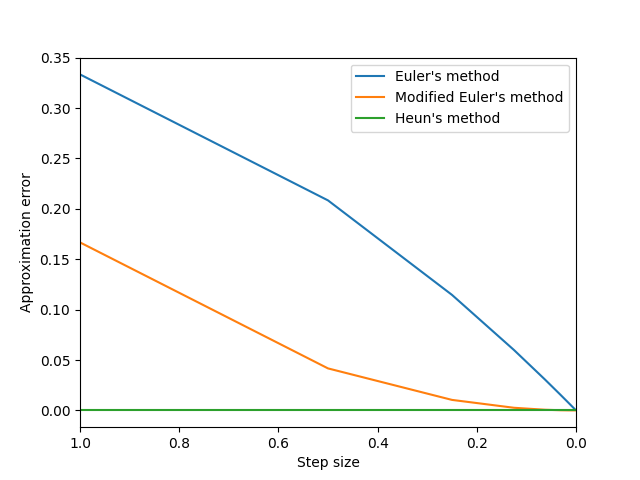
\includegraphics[width=\linewidth]{graph.png}
          \end{center}
          As shown in the plot, the approximation error in both Euler's method and Modified Euler's method decreases as expected, with Modified Euler's method converging faster. Heun's method is exact for this IVP (even for $h=1$, which has a corresponding error of about $10^{-16}$); as a result, the error actually increases slightly as $h$ decreases as rounding error increases.
    \item [5.2.17]
          \begin{itemize}
              \item [(a)] $p(t)=\dfrac{x_n(t)}{x(t)}\implies\dfrac{dp(t)}{dt}=\dfrac{x(t)\cdot\frac{dx_n(t)}{dt}-x_n(t)\cdot\frac{dx(t)}{dt}}{x(t)^2}$\\$=\dfrac{x(t)\cdot[(b-d)x_n(t)+rb(x(t)-x_n(t))]-x_n(t)\cdot[(b-d)x(t)]}{x(t)^2}$\\$=\dfrac{(b-d)x(t)x_n(t)-(b-d)x_n(t)x(t)+x(t)\cdot rb(x(t)-x_n(t))}{x(t)^2}$\\$=\dfrac{rbx(t)^2-rbx(t)x_n(t)}{x(t)^2}$\\$=rb-\dfrac{rbx_n(t)}{x(t)}$\\$=rb(1-p(t))$
              \item [(b)] $p(50)\approx\boxed{0.1042109561743075}$ using Heun's method as shown below.
              \begin{verbatim}
def q17b():
    r, b = 0.1, 0.02
    t_0, t_f, y_0, h = 0, 50, 0.01, 1
    def f(t, w): return r*b*(1-w)

    t, y, steps = t_0, y_0, int((t_f-t_0)/h)
    for _ in range(steps):
        y_prev = y
        y = y_prev + h/4*(f(t, y_prev)+3*f(t+2*h/3,
            y_prev+2*h/3*f(t+h/3, y_prev+h/3*f(t, y_prev))))
        t += h
    print(f"y={y}")
              \end{verbatim}
          \end{itemize}
\end{itemize}
\end{document}